\newpage
\section{MTB-UNI v4}

Další komponentou nového systému \gls{mtb} je nový modul typu \gls{mtbuni}.
Tento modul vznikl, aby bylo možné provádět nové instalace systému \gls{mtb}
a rozšiřovat současné instalace o~nové moduly.

\subsection{Základní parametry}

\begin{table}[ht]
	\begin{tabularx}{\textwidth}{lX}
		\toprule
		Vstupy & 16 digitálních vstupů \\
		Výstupy & 16 výstupů v~režimu otevřeného kolektoru, všechny umožňují
		kmitání a~generování \gls{scom} signálu \\
		Napájení & 7–17 V~DC \\
		Adresování & pomocí jumperů \\
		Procesor & ATmega128 \\
		\bottomrule
	\end{tabularx}
	\caption{Základní parametry modulu \gls{mtbuni} v4}
	\label{tab:mtbuni-params}
\end{table}

Aktuální modul \gls{mtbuni} má 16 digitálních vstupů a~16~digitálních výstupů.
Tento počet se autor práce rozhodl zachovat, protože vhodně škáluje pro malé
i~velké železniční stanice na modelových kolejištích.
Současné \gls{mtbuni} a~MTB-TTL moduly používají různé konektory
pro připojení periferií: svorkovnice nebo nasouvací konektory typu
\texttt{PSH}\footnote{Např. \url{https://www.gme.cz/konektor-se-zamkem-psh02-04pg}.}.
Modul \gls{mtbuni} v4 umožňuje variantní osazení jak svorkovnic, tak konektorů
\texttt{PSH}. Tím modul slučuje současné moduly \gls{mtbuni}, MTB-UNIm a
MTB-TTL do jediné \gls{dps}, což zjednodušuje údržbu a~vývoj.

Hardwarové řešení výstupů je ponecháno: výstupy jsou v~režimu otevřených
kolektorů, jsou řízeny skrze obvody \texttt{ULN2803}, které umožňují
dostatečný výstupní proud až 0.5~A~/~8 výstupů. Všechny výstupy umožňují kmitání
i~vysílání signálu \gls{scom}.

Modul obsahuje 16 digitálních vstupů. Podporu \gls{ir} čidel řeší samostatná
deska, viz \ref{sec:irdet}.

Deska plošných spojů je navržena tak, aby byly zachovány rozměry a~umístění
upevňovacích otvorů se současným nejmenším modulem – MTB-TTL.

Návrh této desky vznikal ve spolupráci s~MENDELU. Schéma vytvořil Robert Čížek,
\gls{dps}, firmware a~koncepční návrh modulu jsou dílem autora této práce.


\subsection{Hardware}

Při návrhu modulu připadají v~úvahu dva přístupy:

\begin{compactenum}
\item malý procesor, posuvné registry na vstupy a~výstupy;
\item velký procesor, vstupy a~výstupy připojené přímo na piny procesoru.
\end{compactenum}

Autor této práce zvolil přístup (2), protože chtěl minimalizovat počet
součástek na desce a~protože v~dnešní době jsou malé procesory s~větším počtem
IO pinů již běžně dostupné.

Schéma i~\gls{dps} jsou vytvořeny v~programu \textit{Eagle} jako openhardware
projekt, dostupné
online\footnote{\url{https://github.com/kmzbrnoI/mtb-uni-4-ele}}, schéma také
v~příloze \ref{fig:mtb-uni-4-sch}. Okomentujme nyní zajímavé prvky schématu
a~\gls{dps}.

Jádrem modulu je procesor \textit{ATmega128}. Autor této práce si zvolil
procesor architektury \textit{AVR}, protože s~používáním těchto procesorů má
dlouholeté zkušenosti. Model \textit{ATmega128} byl pak zvolen proto, že je to
nejmenší model rodiny \textit{ATmega}, který obsahuje požadované množství pinů.

\subsubsection{\textbf{Vstupy}}

\gls{mtbuni} v4 modul oproti modulu současnému obsahuje řádnou ochranu vstupů.
Ochranný obvod vznikl ve spolupráci Jana Horáčka, Michala Petrilaka a~Roberta
Čížka. Zapojení jednoho vstupu je demonstrováno na obrázku \ref{fig:mtbuni-input}.

\begin{figure}[ht]
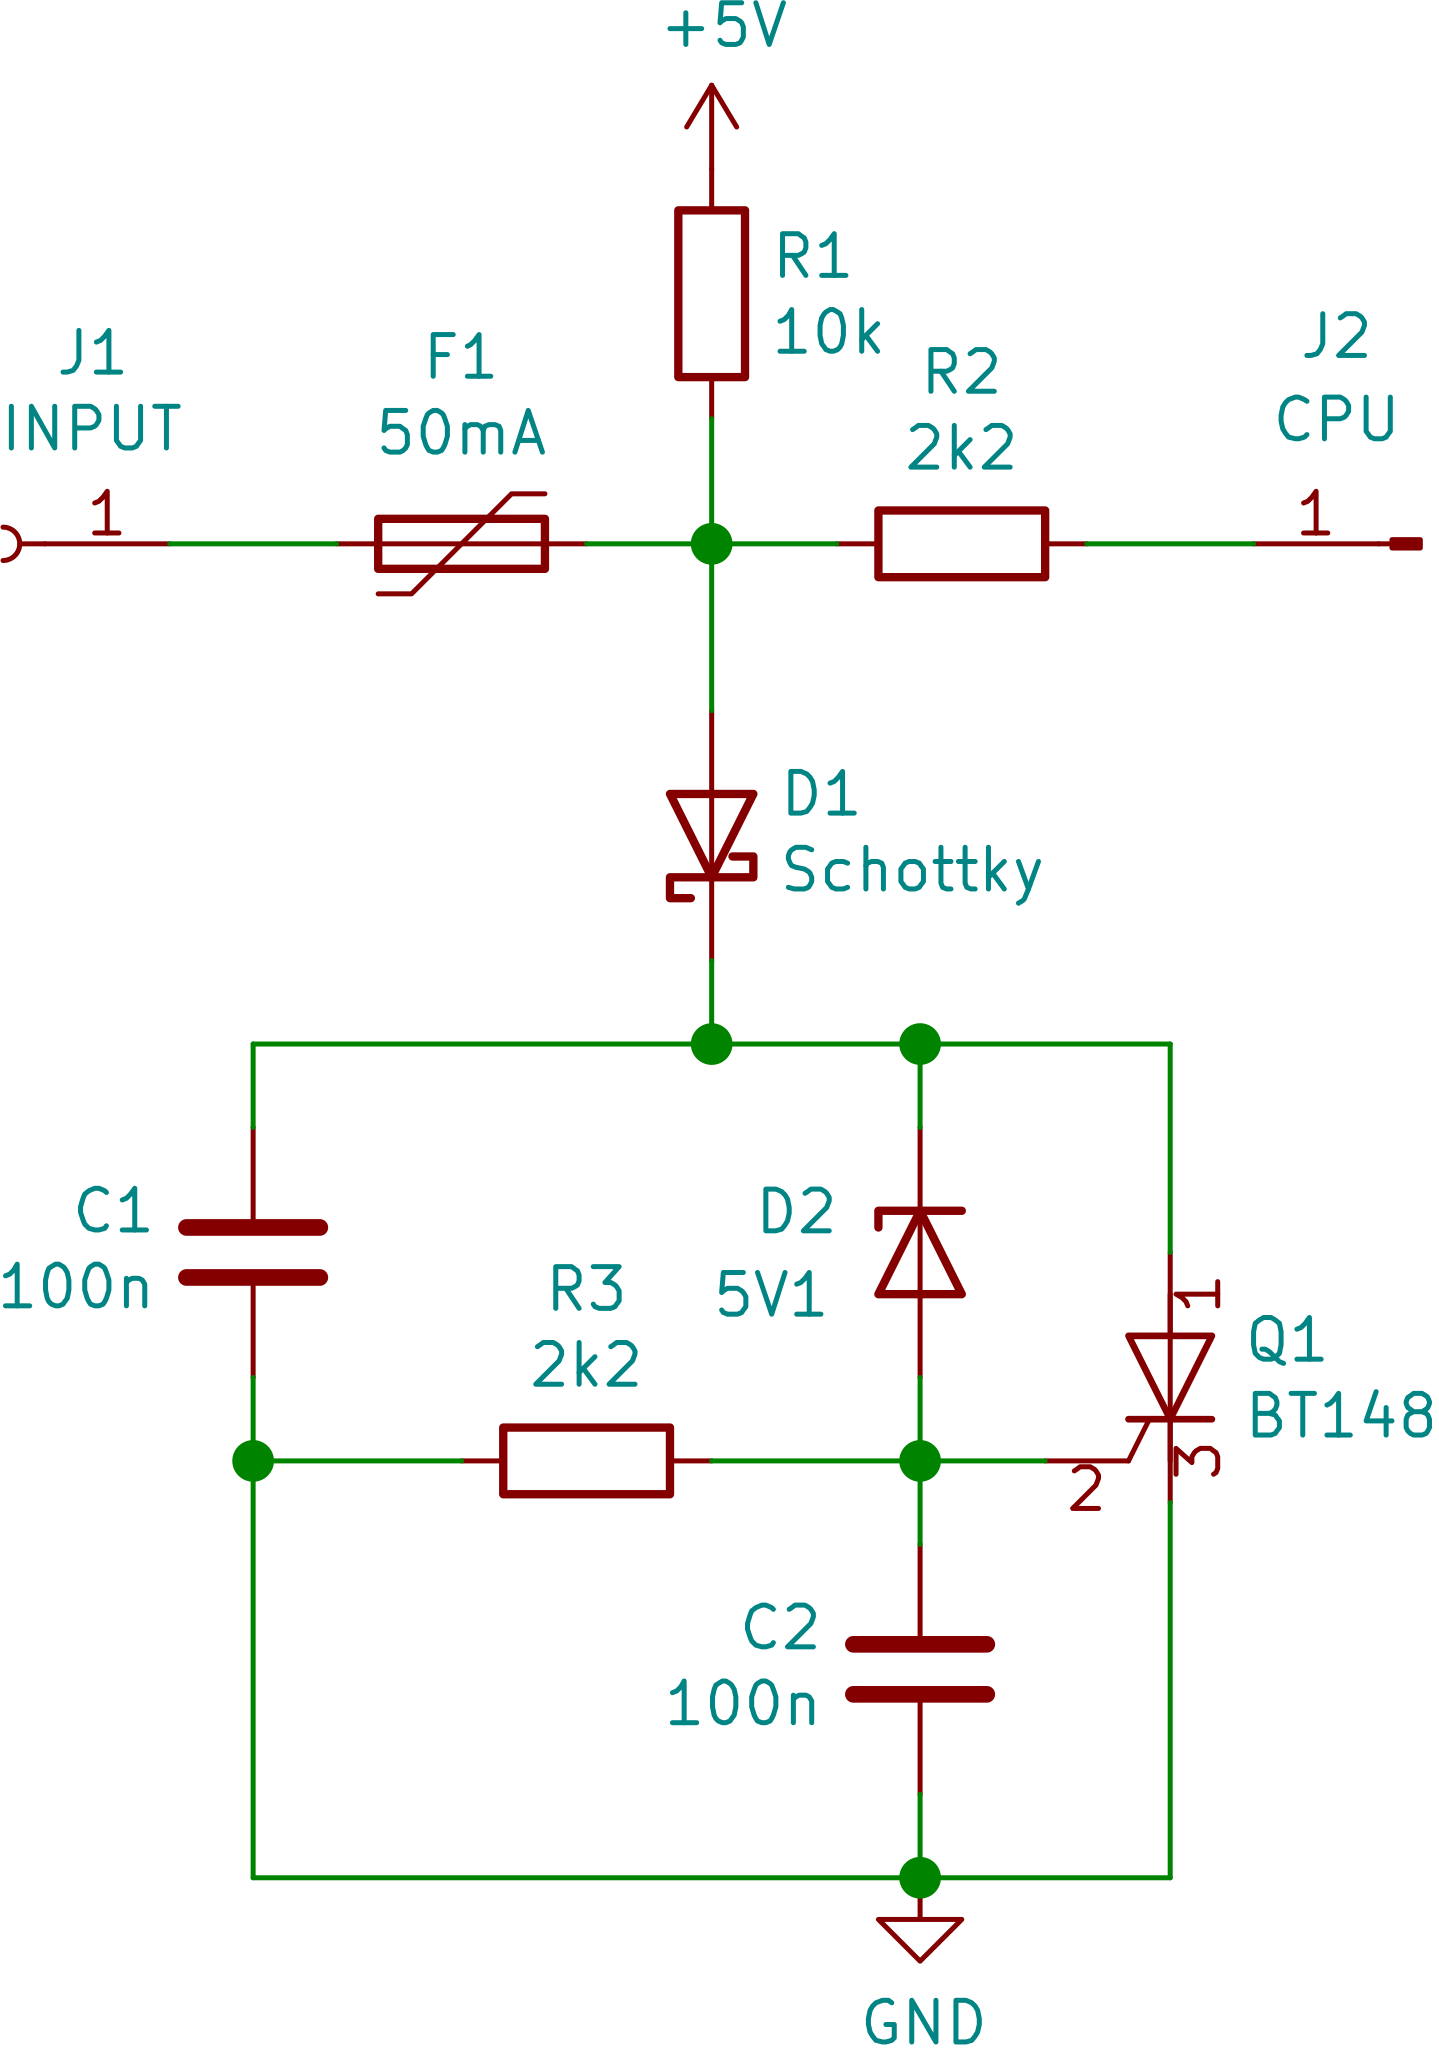
\includegraphics[width=0.4\textwidth]{data/uni-input/uni-input.pdf}
\caption{Zapojení vstupu modulu MTB-UNI.}
\label{fig:mtbuni-input}
\end{figure}

Schéma \ref{fig:mtbuni-input} je rozděleno na 2 části Schottkyho diodou
\texttt{D1}. Horní část včetně diody \texttt{D1} je pro každý z~16 vstupních
pinů zvlášť, spodní je vždy pro osmici pinů společná.

Očekává se, že periferie připojená k~pinu (\texttt{INPUT}) bude tento pin
uzemňovat, případně že bude pin v~režimu \gls{ttl}. Každý vstup obsahuje
pull-up rezistor \texttt{R1}, aby měl vstupní signál vždy definovanou napěťovou
úroveň. Pull-up rezistor je relativně tvrdý, aby se zabránilo ovlivňování
vstupů okolním rušením, které generuje signál \gls{dcc} při přenášení větších
proudů.

K~procesoru vede signál přes ochrannou pojistku \texttt{F1} a~ochranný rezistor
\texttt{R2}. Tento rezistor zabraňuje nadproudu do pinu procesoru a~tím jeho
zničení.

Funkcí celého obvodu od \texttt{D1} níže je vyzkratovat vstup na \textit{GND} v~momentě,
kdy je na něj přivedené vyšší než dovolené napětí. Pin procesoru povoluje
napětí nejvýše $5.5~V$ \cite{atmega128a-datasheet}. Jakmile se vstupní napětí
začne blížit $5.4~V$ ($5.1~V$ Zenerova dioda \texttt{D2} + $0.3~V$ Schottkyho
dioda \texttt{D1}), začne se dioda \texttt{D2} otevírat a~tím začne spínat
i~tyristor \texttt{Q1}.\footnote{V praxi tato situace nastává už při trochu
nižším napětí, cca $5.3~V$, protože pro sepnutí \texttt{Q1} stačí, aby se
\texttt{D2} otevřela jen nepatrně.} Vstupní proud proteče přes \texttt{Q1} do
\textit{GND} a~tím je vstup zkratován. Proud je limitován pojistkou \texttt{F1}.
Tyristor \texttt{Q1} je dimenzován jako výkonový, protože přes něj může téct zkratový
proud všemi 8~piny, navíc chování polymerové pojistky umožňuje krátkodobé řádově
větší proudy, které musí tyristor zvládnout.

V~praxi se často používá zapojení \textit{vstup – ochranný rezistor – pull-up –
pin procesoru}. V~zapojení \gls{mtbuni} desky se oproti tomu používá zapojení
\textit{vstup – pull-up – ochranný rezistor – pin procesoru}. Výhodou zapojení,
které bylo implementováno do \gls{mtbuni} modulu, je, že na vstupu procesoru
není napěťový dělič. V~případě, že vstup má například napětí $0.7~V$ (což se
snadno stane například tehdy, když periferie používá výstupy typu otevřené
kolektory), je toto napětí přivedeno přímo na pin procesoru a~tedy spolehlivě
detekováno jako logická jednička\footnote{V~\gls{mtbuni} je detekováno
jako logická jednička, protože modul používá inverzní logiku.}. Při zapojení
prvního typu by na pinu procesoru vznikl napěťový dělič, který by mohl ohrozit
spolehlivost čtení logického stavu pinu.

\subsubsection{\textbf{Výstupy}}

Na výstupech se používají již zmíněné obvody \texttt{ULN2803}. Za obvody
je vřazena polymerová pojistka. Protože obvod \texttt{ULN2803} specifikuje
proudové omezení $0.5~A$ / všechny výstupy \cite{uln2803-datasheet}, nemohou
samostatné pojistky na jednotlivých výstupech zajistit nepřetížení obvodu
a~zároveň umožnit využití maximálního proudu. Proto jsou na \gls{dps}
\gls{mtbuni} v4 obvody \texttt{ULN2803} jako jedny z~mála osazeny v~paticích
v~\textit{\gls{dil}} provedení.

Výstupy obsahují ochranu proti přivedení vysokého napětí, kterou realizuje
stejný obvod, jako na obrázku \ref{fig:mtbuni-input} (obvod pod diodou
\texttt{D1}). Obdobný obvod realizuje také ochranu proti vysokému napájecímu
napětí celého modulu. Viz kompletní schéma \ref{fig:mtb-uni-4-sch}.

\subsubsection{\textbf{Adresování}}

Adresa modulu \gls{mtbuni} v4 je určena jumpery na modulu. Při návrhu modulu
vznikla diskuze, jaký je nejlepší způsob adresování modulů, přičemž soupeřily
přístupy:

\begin{compactenum}
\item modul má adresu uloženou v~EEPROM, adresu je možné změnit přes \gls{mtbbus},
\item adresa se konfiguruje přímo jumpery na modulu.
\end{compactenum}

Druhý přístup, který zvolil autor této práce, si vysloužil mnohou kritiku.
Autor si však stojí za tím, že snadná a~především vždy pravdivá identifikace
adresy modulu prostým pohledem stojí za 8~vstupních pinů procesoru navíc.

Pro elegantní řešení přístupu (1) je třeba mít na desce tlačítko, kterým se
spouští změna adresy. Tlačítko se na desce nachází, takže pokud by byla
v~budoucnu snaha přejít na přístup (1), je změna otázkou změny firmwaru.

\subsection{Deska plošných spojů}

\gls{dps} je navržená tak, aby byly zachovány rozměry a~umístění
upevňovacích otvorů se současným nejmenším modulem – MTB-TTL. Deska je
dvouvrstvá, používají se primárně SMD součástky velikosti \textit{0805} umístěné
na spodní straně desky (aby bylo možné \gls{dps} automaticky osazovat). Na
obrázku \ref{fig:mtb-uni-v4} lze vidět prototyp desky \gls{mtbuni} v4.0.
Poslední verzí je v4.2, která oproti 4.0 obsahuje více \gls{smd}
součástek a~opravuje chyby prototypu.

\begin{figure}[ht]
\includegraphics[width=0.9\textwidth]{data/uni-v40-screw-all.jpg}
\caption{\gls{mtbuni} v4.0.}
\label{fig:mtb-uni-v4}
\end{figure}

\subsection{Firmware}

Firmware pro procesor \textit{ATmega128} je psán v~jazyce \texttt{C} a~je
dostupný pod opensource licencí
online\footnote{\url{https://github.com/kmzbrnoI/mtb-uni-4-fw}}.

Zajímavým prvkem firmwaru je podpora jeho aktualizace přímo přes \gls{mtbbus}.
Firmware obsahuje dvě části:

\begin{compactenum}
\item hlavní program,
\item bootloader.
\end{compactenum}

Bootloader je ve speciální části paměti (na konci) a~zajišťuje
aktualizaci hlavního programu. Bootloader je měnitelný pouze přímým
programováním procesoru, nikoliv přes \gls{mtbbus}. Firmware tak v~zásadě
obsahuje 2 samostatné programy, které se po zkompilování slinkují dohromady.

Bootloader umí pouze aktualizovat firmware a~kontrolovat jeho konzistenci.
Kontrola konzistence firmwaru je implementována pomocí uložení CRC-16
kontrolního součtu a~počtu aktivních stránek paměti na konkrétních adresách
paměti (na konci těsně před bootloaderem).
